\documentclass[10pt,stdletter,dateno,sigleft]{newlfm} % Extra options: 'sigleft' for a left-aligned signature, 'stdletternofrom' to remove the from address, 'letterpaper' for US letter paper - consult the newlfm class manual for more options

\renewcommand{\rmdefault}{phv} % Arial
\renewcommand{\sfdefault}{phv} % Arial

\usepackage{charter} % Use the Charter font for the document text
\usepackage{hyperref} 
\hypersetup{colorlinks,breaklinks,urlcolor=blue,linkcolor=blue}


\newsavebox{\Luiuc}\sbox{\Luiuc}{\parbox[b]{1.75in}{\vspace{0.2in}
% Company/institution logo at the top left of the page
%\includegraphics[width=0.6\linewidth]{myLogo.png}
}}
\makeletterhead{Uiuc}{\Lheader{\usebox{\Luiuc}}}

\newlfmP{sigsize=50pt} % Slightly decrease the height of the signature field
\newlfmP{addrfromphone} % Print a phone number under the sender's address
\newlfmP{addrfromemail} % Print an email address under the sender's address
\PhrPhone{Phone} % Customize the "Telephone" text
\PhrEmail{Email} % Customize the "E-mail" text

\lthUiuc % Print the company/institution logo

\newenvironment{nopgbrk}
{\par\nobreak\vfil\penalty0\vfilneg
\vtop\bgroup}
{\par\xdef\tpd{\the\prevdepth}\egroup
\prevdepth=\tpd}
%----------------------------------------------------------------------------------------
%	YOUR NAME AND CONTACT INFORMATION
%----------------------------------------------------------------------------------------

%\namefrom{Rafael P\'erez} % Name

\addrfrom{
\today\\[12pt] % Date
238 Oceana Boulevard \\ % Address
Southampton UK, SO14 3JG
}

\phonefrom{+44 (0) 744 954 9630} % Phone number
\emailfrom{rpereztorro@gmail.com} % Email address

%----------------------------------------------------------------------------------------
%	ADDRESSEE AND GREETING/CLOSING
%----------------------------------------------------------------------------------------

\greetto{Dear Sir or Madam,} % Greeting text
%\closeline{Yours Faithfull,}


\nameto{} % Addressee of the letter above the to address

\addrto{
Renault UK Ltd \\
The Rivers Office Park, \\
Denham Way, \\
Maple Cross, \\
Rickmansworth (Hertfordshire), WD3 9YS (UK)\\
\\
Job reference: \textbf{RSR-AER43 -- Thermodynamics CFD Engineer}  
}

%----------------------------------------------------------------------------------------

\begin{document}
\begin{newlfm}

%----------------------------------------------------------------------------------------
%	LETTER CONTENT
%----------------------------------------------------------------------------------------

I am writing this letter in response to the ``Thermodynamics CFD Engineer'' job advert on
RenaultSport's website for which I believe I have the appropriate set of skills. 

I am currently finishing (this November) a PhD on the topic of Large-Eddy-Simulations of
wings with leading-edge modifications, and I am looking to take this further on my next
career challenge. After finishing my MSc in Race Car Aerodynamics I felt myself prepared to take
on a position such as the one now in consideration. However, after three years in the
research field, not only have I enhanced my previous skills but also acquired new
ones. A side from enhancing my knowledge, the PhD has made me more independent, being able
to quickly find solutions to specific problems. All in all, research has expanded my
knowledge and expertise to such an extent that I am able to meet expectations to a higher
degree and fight for each millisecond in each lap.

Additionally, although the research experience has been very rewarding, I feel that due to
my competitive character, I would much rather continue developing my career in the
fast-paced and team-based working environment of a F1 team.

Thank you for your time and consideration and please feel free to contact me, or visit my
linkedin profile (\href{https://uk.linkedin.com/in/rperezt}{uk.linkedin.com/in/rperezt})
if you need any more details.

Yours Faithfully, \newline % Closing text
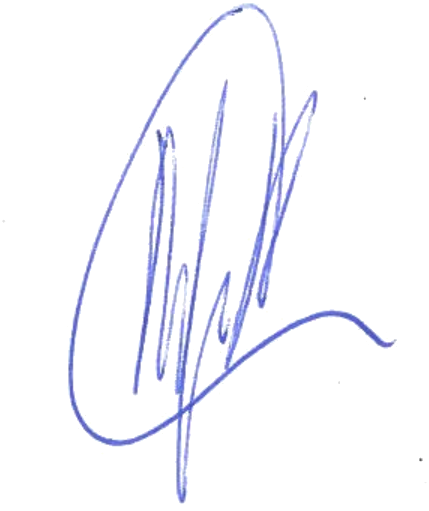
\includegraphics[scale=0.6]{sgtrBlue} \newline 
Rafael P\'erez

%----------------------------------------------------------------------------------------

\end{newlfm}
\end{document}
